\documentclass[titlepage]{article}
\usepackage{amsmath}
\usepackage[utf8]{inputenc}
\usepackage{graphicx}

\author{Jan Alexander Bremnes\\Magnus Kirø}
\title{IT3105 - Ex 2\\Voice Recognition}
\date{September 2011}

\begin{document}

    \maketitle
    \tableofcontents
    \pagenumbering{arabic}
    \graphicspath{{SRS/img/}}
    \newpage

\section{Introduction}
In this report we will discuss the process of speech recognition, a project in the course IT3105 - AI programming. We start out with four words in our vocabulary (start, stop, left, right) and a set of testing words. The goal of this exercise is to classify the input as one of the words in our vocabulary. To achieve this we use hidden Markov models(HMM) as a key component in our calculations. HMMs are common in spech recognition, and quite usefull in many other cases. 

In the first part we read the sound files(.wav), devide the datastructure for the sound data and finds characteristics about the specific sound file with basic operations for sound files. 

Part two is basicly the classification of sound. Checking if the input matches some of the words in our vocabulary. To achieve this we have to define the HMM and implement the classifier, that works as an umbrella for the different HMM models. 

Part three is the part of learning. Here we use the starting set of sound files to optimize the HMM precision. Thus learning through the iterations of starting set of data. 

Part four, testing and polishing. The part where we find out if we have done something right. We are to run the test data and classify the sounds there as words. And tweaking the our parameters for calculation in order to improve our classification rate.  

\section{System Description}

\subsection{Overall Description}

\subsection{Code Files and what they do}
\begin{itemize}
\subsubsection{Main} \item[main.m] Main contains two functions. the createSRS function and the recognize function. The recognize function contains the code for reading the test files, the file that is to be classified later. Recognize simply reads input data and asks classify to return the word that is most likely to be the input word. The createSRS function trains the model, the HMM, to be more specific. This in turn increases the chance of recognizing a word. This is done 
\subsubsection{Data} \item[data.m] Data contains the code to manipulate the data from the .wav files to a more useful representation. Fist we find the length of the window we want to use and normalize the input sound data before we create the matrix of frames with 80 samples per fram and 50percent overlap. Then we fourier transform the framed signal. While doing the fourier transform we also smooth it out with the hamming window. Then we use findpeaks to specify points of data to identify the specific word. We use findpeaks for each frame.  
\subsubsection{Classifier}\item[classifier.m] The constructor of this class takes the vocabulary we have and stores it in the class. The classify function in the classifier class gets called with the data to be compared to the vocabulary. Classify calls the forwardHMM with the data to be classified and the model it is being compared to. FOrwardHMM then returns the probability of likelihood. Classify finds the highest probability and returns the corresponding word.  
\subsubsection{HMM}\item[HMM.m] The model in which we store data.

\subsubsection{forwardHMM}\item[forwardhmm.m] ForwardHMM 
\subsubsection{backwardHMM}\item[backwardhmm.m] df
\subsubsection{calcLikelihood}\item[calcLikelihood.m] Calculates the proability of one 
\subsubsection{Learn}\item[learn.m] The training code.   

\end{itemize}


\section{Data Representation}
% How we represent the sound as data and why. 
% Results from the different parts si required. 
    % picture from part 1
    % picture from part 2
    % picture from part 3
    % picture from part 4
    \subsection{Sound files .wav} 
When the .wav files are read in Matlab they are represented in a one dimensional array with doubles. e.g: [-0.0131; -0.0073; 0.0010; 0.0125]
    \subsection{Data Structure}
The prepared data has a complex structure. The matrix becomes a <5x2xno.frames double>. We have lots of frames with a list of peaks and a list of locations. Peaks and locations have five entries each. Thus we get <peak entries in, peaks and locations, for all the frames>. 

We split our data in to chunks, frames, to get precision and enugh data to make comparisons. for each frame we find peaks in the data. This is after the fourier transformation is done, so we have a smooth graph with data points. All the individual frames can be combined to make one graph representing all the data. 
%img og the a graph representing the data.

We find datapoints, peaks, to represent the data from each frame. We considered to use peakdet, but decided to use findpeaks. Findpeaks finds all points where the closest two points to itself is lower then itself. Then we store the five highest peaks in our datastructure, in peaks and locations(x and y of the peak) in our datastructure. The five stored peaks are the most significant peaks for the given frame. 

We chose this structure for our data to be able to have all the data in one matrix. This makes operations on our structure easy with the matrix operations in Matlab. We thought of using spectrograms early in the poject, but rejected them because we didn't find an easy way to use them. 

\begin{figure}[Data Structure]
  \centering
    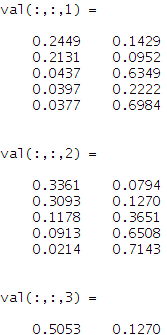
\includegraphics[height=60mm\textwidth]{data_part1}
  \caption{Frame 1, 2 and part of 3. From the returned data of the data preparation procedure. W can see that we have five values in each column. The columns area peaks and locations.}
\end{figure}

    \subsection{HMM}

  
\section{Test data classification and results}
% picture or table of the classification results. 


\section{Project Parts}
	\subsection{Part 1 - Input and Data Structure}
\begin{itemize}
\item Read .wav-files (Matlab-command: wavread) and play the sound (Matlabcommand: sound).
\item Partition time-series data into partly overlapping frames (Matlab-command:
buffer), and windowing (Matlab-command: hamming).
\item Extract the spectral density of the signal for each frame (Matlab-command:
fft, see also spectrogram). If required: Extract the complex cepstral parameters from the signal inside each frame (Matlab-command: cceps).
\end{itemize}

	\subsection{Part 2 - Classification and Framework}
\begin{itemize}
\item The hmm class, which implements the Hidden Markov models with assorted inference mechanism.
\item The classifier class, which implements the wrapping of the instances of the hmm class, takes care of the data flow, and the top-level calculations
\end{itemize}	

    \subsection{Part 3 - Learning}
Learning one HMM per word. 
\begin{itemize}
\item 1. Concatenate all the speech signals representing utterances of a particular word into a “huge” file.
\item 2. Generate feature description of the “huge” file (called the feature-file).
\item 3. Choose parameters in the HMM to maximize the probability of observing exactly the observations in the feature-file. The maximization can be done using the EM-algorithm, see the lecture notes.
\end{itemize}

    \subsection{Part 4 - Testing and Tweaking. }
\begin{itemize}
\item Learn one HMM per word in the vocabulary. You should use all the files of the type <word> <number>.* for learning each model.
\item Test your system by classifying all the examples query <number>.* and report classification accuracy.
\item To obtain as good results as possible, you can tune the number of states in the hidden variable and also re-investigate how to represent sounds (Part I). It is expected that your system classifies at least 50percent of unseen examples correctly.
\end{itemize}



%%stolen stuff to read.

\section{Introduction}
The following document is a report for the project \emph{speech recognition} of the course IT3105. The goal was to build up a simple speech recognition system (SRS) with limited vocabulary. Namely 4 words (\emph{start, stop, left, right}). Our calculation should rely on \emph{hidden Markov models} (HMM), a quite common method in speech recognition. For that we had to take several steps. In the first one a input soundfile had to be captured. From that robust feature vectors for several frames of the signal had to be computed. The second part contained the implementation of the HMM, the calculation algorithm and the framework for connecting all these parts. In the last part the task was to apply learning to our system in order to optimise the parameters. Detailed information on every part may be found in the following sections.

As implementation tool for the project we used MATLAB and its programming language. We followed this recommendation in face of the fact that the implementation was going to be related to signal processing and matrix calculations. Both, fields in which MATLAB is extraordinary powerful.

\section{System Description}\label{sec:system}
The interface of our SRS is provided by a function called \lstinline&recognize&. That takes as argument the path of the soundfile that has to be recognized and gives back a text representation of the word found by the system. The function is actually very small, because it basically just starts the bigger parts of the system. So after reading the sound data from a wav-file with the MATLAB built-in function \lstinline&wavread& these data are processed in a function called \lstinline&dataPrep&. That is the part where the preparation for the following recognition process happens (see section \ref{sec:prep}).
Like it is suggested in the project notes we built a class \lstinline&classifier& that acts like a frame around the recognition process. We instantiate an object of \lstinline&classifier&. As already mentioned in the introduction we use hidden Markov models to model our vocabulary. That means we use one HMM for each word. Therefore there is a class \lstinline&hmm& and the classifier holds 4 objects of this (more in section \ref{sec:hmm}). On the classifier we call its function \lstinline&classify& which checks every model and compares their probabilities to model the really recorded word and give back the word of the model with the highest probability.

%part for something on learning

\section{Data Preparation}\label{sec:prep}
As already mentioned before the data preparation happens in the function \lstinline&dataPrep& which has as arguments the vector of signed floating-point numbers (\lstinline&data&), representing the sound signal, and its sampling rate (\lstinline&Fs&). The function starts with setting the length of frames. As suggested we use $1/100 s$, i.e. 80 samples per frame for a sampling rate of 8000 Hz. Before the signal is framed it gets normalised so that the maximum amplitude is set to 1. The framing happens with the built-in function \lstinline&buffer&. The overlapping is set to 50\%. After that we apply the fast Fourier transformation (FFT) to each frame to get the spectrum and thus a more robust representation of the sound signal. Since the spectra are still complex we calculate the absolute value. From that we extract the 5 greatest values and their associated frequencies (normalised) for each frame and store them in a matrix. All these matrices are stored in an array which means, in fact, that we a kind of stack of 5x2-matrices. The height of this stack depends on the number of frames. This stack is returned from the function to be processed further in the recognition. An example for a computation on one frame may be seen in figure \ref{fig:frame}.

\begin{figure}[htbp]
	\centering
		\subfigure[][Signal in time domain]{\includegraphics[width=0.7\textwidth]{signal.jpg}}
		\subfigure[][Spectrum (blue) and extracted features (red crosses)]{\includegraphics[width=0.7\textwidth]{spectrum.jpg}}
	\label{fig:frame}
	\caption{Frame 2 of file \lstinline&stop_1.wav&}
\end{figure}

\section{Recognition Framework}\label{sec:hmm}
Part two of the project was the building of the basic recognition system except of filling it with wise values for the different models (for that see section \ref{sec:learn}). The recognition system is basically encapsulated in the class \lstinline&classifier&, like already discussed in section \ref{sec:system}. The core of the recognition lays in the HMMs which are realised in a class \lstinline&hmm&. In the design we followed the suggestion from the project notes as well as we took over the \lstinline&forwardHMM& function with just one or two adjustments, for example, the return of matrix \textbf{B} (used for learning). In there a \lstinline&calcLikelihood& called function is used to calculate the likelihood of the observed data. This function applies a multivariate normal (Gaussian) distribution (no mixture of several distributions) to every feature entry. That means we get one likelihood for each feature. These likelihoods are added up weighted, so that the likelihood of the greatest magnitude in the spectrum influences most.


\section{Learning}\label{sec:learn}
To have a working SRS the learning of the models must apparently happen before. So before we start the classifier we generate our vocabulary (matrix of HMM) and pass it through a function called train-model. That function takes the whole data set that is provided for learning. This data set is sent to another function called learn which is the basic implementation of the learning algorithm. In there the steps a)-e) are applied to the HMM except of d) since we do not use a mixture of Gaussian distributions. The implementation is basically just writing down the formulas showed in the paper.

\end{document}
